\documentclass{standalone}
\usepackage{amsmath,scalerel}
\usepackage{tikz}

\begin{document}
	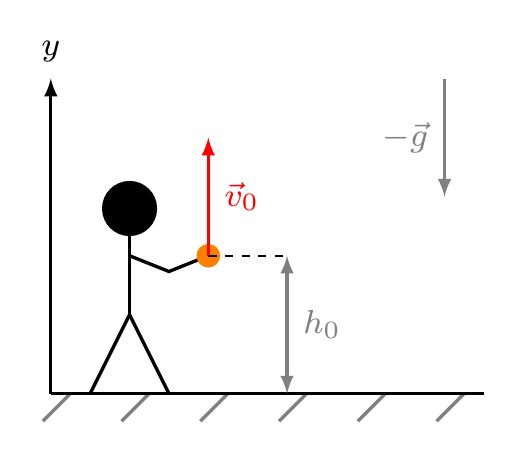
\begin{tikzpicture}
		[
		x=1cm, y=1cm, scale=1.0, font=\footnotesize, >=latex 
		%Voreinstellung für Pfeilspitzen
		]
		
		%Raster im Hintergrund
		%\draw[step=1, gray!50!white, very thin] (-2,-2) grid (5,5);
		
		%Zahlen auf x-Achse
		\foreach \x in {-0.75,0.25,1.25,2.25,3.25,4.25}
		\draw[shift={(\x,0)},color=gray, very thick] (0pt,0pt) -- (-10pt,-10pt);
		
		\draw [very thick] (0.5,0)--(0,1);
		\draw [very thick] (-0.5,0)--(0,1);
		\draw [very thick] (0,1)--++(0,1);
		\draw [very thick] (0,1.75)--(0.5,1.55)--(1,1.75);
		\fill (0,2.35) circle (0.35);
		\fill [orange](1,1.75) circle (0.15);
		%Länge x Achse
		\draw [thick] (-1,0) -- ++(5.5,0);
		\draw [-latex, very thick, red] (1,1.75)--++(0,1.5) node [midway, right, red, xshift=0pt, yshift=0pt, scale=1.5] {$\vec{v}_0$} {};
		\draw [-latex, very thick, gray] (4,4)--++(0,-1.5) node [midway, left, gray, xshift=0pt, yshift=0pt, scale=1.5] {$-\vec{g}$} {};
		\draw [-latex, very thick] (-1,0)--++(0,4) node [above, xshift=0pt, yshift=0pt, scale=1.5] {$y$} {};
		\draw [<->, very thick, gray] (2,0)--++(0,1.75) node [midway, right, gray, xshift=0pt, yshift=0pt, scale=1.5] {$h_0$} {};
		\draw [dashed, thick] (1,1.75)--++(1,0);
	\end{tikzpicture}

\end{document}